\documentclass[aspectratio=169,xcolor={dvipsnames,table}]{beamer}
\usepackage[no-math,deluxe,expert,haranoaji]{luatexja-preset}
\usepackage{luatexja-otf}
\renewcommand{\kanjifamilydefault}{\gtdefault}
\renewcommand{\emph}[1]{{\upshape\bfseries #1}}
\usetheme{metropolis}
\metroset{block=fill}
\setbeamertemplate{navigation symbols}{}
\usecolortheme[rgb={0.7,0.2,0.2}]{structure}
%%%%%%%%%%%%%%%%%%%%%%%%%%%
\usepackage{media9}
%%%%%%%%%%%%%%%%%%%%%%%%%%%
%% さまざまなアイコン
%%%%%%%%%%%%%%%%%%%%%%%%%%%
%\usepackage{fontawesome}
\usepackage{fontawesome5}
\usepackage{figchild}
\usepackage{twemojis}
\usepackage{utfsym}
\usepackage{bclogo}
\usepackage{marvosym}
\usepackage{fontmfizz}
\usepackage{pifont}
\usepackage{phaistos}
\usepackage{worldflags}
\usepackage{jigsaw}
\usepackage{tikzlings}
\usepackage{tikzducks}
\usepackage{scsnowman}
\usepackage{epsdice}
\usepackage{halloweenmath}
\usepackage{svrsymbols}
\usepackage{countriesofeurope}
%%%%%%%%%%%%%%%%%%%%%%%%%%%
\usepackage{tikz}
\usetikzlibrary{backgrounds}
\usepackage{tcolorbox}
\usepackage{tikzpeople}
\usepackage{circledsteps}
\usepackage{xcolor}
\usepackage{amsmath}
\usepackage{booktabs}
\usepackage{chronology}
\usepackage{signchart}
\usepackage{pxrubrica}
\usepackage{tipa}
%%%%%%%%%%%%%%%%%%%%%%%%%%%
%% 場合分け
\usepackage{cases}
%%%%%%%%%%%%%%%%%%%%%%%%%%%
% \myAnch{<名前>}{<色>}{<テキスト>}
% 指定のテキストを指定の色の四角枠で囲み, 指定の名前をもつTikZの
% ノードとして出力する. 図には remeber picture 属性を付けている
% ので外部から参照可能である.
\newcommand*{\myAnch}[3]{%
  \tikz[remember picture,baseline=(#1.base)]
    \node[draw,rectangle,#2] (#1) {\normalcolor #3};
}
%%%%%%%%%%%%%%%%%%%%%%%%%%%%
%% 音声リンク表示
\newcommand{\myaudio}[1]{\href{#1}{\faVolumeUp}}
%%%%%%%%%%%%%%%%%%%%%%%%%%%
% \myEmph コマンドの定義
%\newcommand{\myEmph}[3]{%
%    \textbf<#1>{\color<#1>{#2}{#3}}%
%}
\usepackage{xparse} % xparseパッケージの読み込み
\NewDocumentCommand{\myEmph}{O{} m m}{%
    \def\argOne{#1}%
    \ifx\argOne\empty
        \textbf{\color{#2}{#3}}% オプション引数が省略された場合
    \else
        \textbf<#1>{\color<#1>{#2}{#3}}% オプション引数が指定された場合
    \fi
}
%%%%%%%%%%%%%%%%%%%%%%%%%%%
%% 文末の上昇イントネーション記号 \myRisingPitch
%% 通常のイントネーション \myDownwardPitch
%% https://note.com/dan_oyama/n/n8be58e8797b2
%%%%%%%%%%%%%%%%%%%%%%%%%%%
\newcommand{\myRisingPitch}{
\begin{tikzpicture}[scale=0.3,baseline=0.3]
\draw[->,>=stealth] (0,0) to[bend right=45] (1,1);
\end{tikzpicture}
}
\newcommand{\myDownwardPitch}{
\begin{tikzpicture}[scale=0.3,baseline=0.3]
\draw[->,>=stealth] (0,1) to[bend left=45] (1,0);
\end{tikzpicture}
}
%%%%%%%%%%%%%%%%%%%%%%%%%%%
\makeatletter
\newcommand*{\themonth}{\two@digits\month}
\newcommand*{\theday}{\two@digits\day}
\makeatother
\newcommand{\mytoday}{{\the\year}--{\themonth}--{\theday}}
%%%%%%%%%%%%%%%%%%%%%%%%%%%
%%%%%%%%%%%%%%%%%%%%%%%%%%%
\title{English is fun.\,\,{}--- I have lost my bag. ---}
  \author{}
\institute[]{}
\date[]

%%%%%%%%%%%%%%%%%%%%%%%%%%%%
%% TEXT
%%%%%%%%%%%%%%%%%%%%%%%%%%%%
\begin{document}
%%%%%%%%%%%%%%%%%%%%%%%%%%%
\setbeamercolor{background canvas}{bg=black}
\begin{frame}
%\centering
\raggedleft
  \textcolor{white}{\Huge\bfseries English is fun.}

\vfill

\raggedleft
% \textcolor{white}{\LARGE\bfseries 2024--11--26}
% \textcolor{white}{\LARGE\bfseries \today}
 \textcolor{white}{\LARGE\bfseries \mytoday}

\vfill
\vfill
\vfill

\raggedleft
\textcolor{white}{\large The lesson will begin at the scheduled time.}

%\textcolor{white}{\large 可能なら、鏡を用意してください}
\end{frame}
\setbeamercolor{background canvas}{bg=}
%%%%%%%%%%%%%%%%%%%%%%%%%%
%%%%%%%%%%%%%%%%%%%
%%% youtube
%%%%%%%%%%%%%%%%%%%%%%%%%%%%%%%%%%%%%%%%%%%%%%%%%%%%%
% 背景色をグレイに変更
%\setbeamercolor{background canvas}{bg=gray}
\setbeamercolor{background canvas}{bg=black}

\begin{frame}
%\centering
\raggedleft
  \textcolor{white}{\Huge\bfseries \textcolor{yellow}{E}nglish is fun.}

\vfill

\vfill

\raggedleft
 \textcolor{white}{\LARGE\bfseries \textcolor{yellow}{H}ello, everybody!}

 \textcolor{white}{\LARGE\bfseries \textcolor{yellow}{H}ow are you today?}

\raggedleft
 \textcolor{white}{\LARGE\bfseries \textcolor{yellow}{A}re you ready to start?}

 \textcolor{white}{\LARGE\bfseries \textcolor{yellow}{L}et's begin today's lesson.}

\vfill

\raggedleft
% \textcolor{white}{\LARGE\bfseries 2024--11--26}
% \textcolor{white}{\LARGE\bfseries \today}
 \textcolor{white}{\Large \bfseries \mytoday}

\end{frame}
%%%%%%%%%%%%%%%%%%%%%%%%%
\begin{frame}[plain]
 \centering

\Huge

\textcolor{white}{\textbf{Catch the Alphabet!}}

\raggedleft
\hyperlink{today_n}{\beamergotobutton{Today's Mission}}%%todayにジャンプ

\end{frame}
%%%%%%%%%%%%%%%%%%%%%%%%%%%%
%% A
%%%%%%%%%%%%%%%%%%%%%%%%%%%%%%%%%%%%%%%%%%%%%%%%%%
\setbeamercolor{background canvas}{bg=}
%%%%%%%%%%%%%%%%%%%%%%%%%%%%%%%%%%%%%%%%%%%%%%%%%
\begin{frame}[plain]{Quiz}
\hypertarget{today_a}{}

 \large
{\small %
これからアルファベットを6つ順番に読みあげます。
聞こえたアルファベットを順番に小文字で書いてください。すると単語になります。その意味を表す図を選んでください
}
\mbox{}\hfill{\tiny 0100}\,{\scriptsize \myaudio{./audio/quiz/quiz_a.mp3}}

\bigskip

\centering
\begin{tabular}{c@{   }c@{   }c@{   }c}
\scalebox{.8}{
\begin{tikzpicture}
\bear
\end{tikzpicture}%
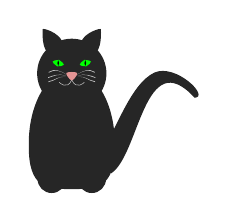
\begin{tikzpicture}
 \cat[eye=green]
\end{tikzpicture}}&
\scsnowman[scale=5,eyes, mouth,
nose, arms, hat=NavyBlue, muffler=Maroon,
buttons, snow, broom]&
\scalebox{6}{\twemoji{sushi}}&
\scalebox{6}{\twemoji{lemon}}\\
(a)&(b)&(c)&(d)
\end{tabular}
\bigskip

\Huge

\onslide<2->{a}%
\onslide<3->{n}%
\onslide<4->{i}%
\onslide<5->{m}%
\onslide<6->{a}%
\onslide<7->{l}%

\large
\mbox{}\hfill{\tiny 0038}\,{\scriptsize \myaudio{./audio/quiz/answer_a.mp3}}
\end{frame}
%%%%%%%%%%%%%%%%%%%%%%%%%%%%%%%%%%%%%%%%%%%%%%%%%%
%% B
%%%%%%%%%%%%%%%%%%%%%%%%%%%%%%%%%%%%%%%%%%%%%%%%%%
\begin{frame}[plain]{Quiz}
\hypertarget{today_b}{}

 \large
{\small%
これからアルファベットを4つ順番に読みあげます。
聞こえたアルファベットを順番に小文字で書いてください。すると、ある単語になります。その意味を表す図を選んでください
}
\mbox{}\hfill{\tiny 0048}\,{\scriptsize \myaudio{./audio/quiz/quiz_b.mp3}}

\bigskip

\centering
\begin{tabular}{c@{   }c@{   }c@{   }c}
\fcBike{.7}{Maroon}{1}&
\scalebox{6}{\twemoji{doughnut}}&
\scalebox{6}{\twemoji{sunflower}}&
\scalebox{6}{\twemoji{book}}\\
(a)&(b)&(c)&(d)
\end{tabular}

\bigskip

\Huge

\onslide<2->{b}%
\onslide<3->{o}%
\onslide<4->{o}%
\onslide<5->{k}%

\large
\mbox{}\hfill{\tiny 0037}\,{\scriptsize \myaudio{./audio/quiz/answer_b.mp3}}
\end{frame}
%%%%%%%%%%%%%%%%%%%%%%%%%%%%%%%%%%%%%%%
%% C
%%%%%%%%%%%%%%%%%%%%%%%%%%%%%%%%%%%%%%%%%%%%%%%%%%
\begin{frame}[plain]{Quiz}
\hypertarget{today_c}{}

 \large
{\small%
これからアルファベットを5つ順番に読みあげます。
聞こえたアルファベットを順番に小文字で書いてください。すると、ある単語になります。その意味を表す図を選んでください
}
\mbox{}\hfill{\tiny 0054}{\scriptsize \myaudio{./audio/quiz/quiz_c.mp3}}

\bigskip

\centering
\begin{tabular}{c@{   }c@{   }c@{   }c}
\scalebox{7}{\twemoji{carrot}}&
\scalebox{7}{\twemoji{doughnut}}&
\scalebox{7}{\twemoji{candy}}&
\scalebox{7}{\twemoji{cake}}\\
(a)&(b)&(c)&(d)
\end{tabular}

\bigskip

\Huge

\onslide<2->{c}%
\onslide<3->{a}%
\onslide<4->{n}%
\onslide<5->{d}%
\onslide<6->{y}%

\large
\mbox{}\hfill{\tiny 0038}\,{\scriptsize \myaudio{./audio/quiz/answer_c.mp3}}
\end{frame}
%%%%%%%%%%%%%%%%%%%%%%%%%%%%%%%%%%%%%%%%%%%%%%%%%%
%\begin{frame}[plain]{candy}
%
%\includegraphics[height=.875\textheight]{./images/candy.jpg}
%
%\raggedleft
%\tiny
%"Lollipop 091" by greenbes is licensed under CC BY 2.0.\\
%To view a copy of this license, visit \url{https://creativecommons.org/licenses/by/2.0/?ref=openverse}.
%
%
% \end{frame}
%%%%%%%%%%%%%%%%%%%%%%%%%%%%
%% D
%%%%%%%%%%%%%%%%%%%%%%%%%%%%%%%%%%%%%%%%%%%%%%%%%%
\begin{frame}[plain]{Quiz}
\hypertarget{today_d}{}

 \large
{\small%
これからアルファベットを7つ順番に読みあげます。
聞こえたアルファベットを順番に小文字で書いてください。すると、ある単語になります。その意味を表す図を選んでください
}
\mbox{}\hfill{\tiny 0106}\,{\scriptsize \myaudio{./audio/quiz/quiz_d.mp3}}

\bigskip

\centering
\begin{tabular}{c@{   }c@{   }c@{   }c}
\scalebox{7}{\twemoji{club suit}}&
\scalebox{7}{\twemoji{diamond suit}}&
\scalebox{7}{\twemoji{heart suit}}&
\scalebox{7}{\twemoji{spade suit}}\\
(a)&(b)&(c)&(d)
\end{tabular}

\bigskip
\Huge

\onslide<2->{d}%
\onslide<3->{i}%
\onslide<4->{a}%
\onslide<5->{m}%
\onslide<6->{o}%
\onslide<7->{n}%
\onslide<8->{d}

\large
\mbox{}\hfill{\tiny 0038}\,{\scriptsize \myaudio{./audio/quiz/answer_d.mp3}}
\end{frame}
%%%%%%%%%%%%%%%%%%%%%%%%%%%%%%%%%%%%%%%%%%%%%%%%%%
\begin{frame}[plain]{もちろん、これもdiamondです}
%
\raggedleft
%
\includegraphics[height=.95\textheight]{./images/diamonds.jpg}

\vspace*{-8pt}
\tiny
%
Photo by \href{https://unsplash.com/@edgardo1987?utm_content=creditCopyText&utm_medium=referral&utm_source=unsplash}{Edgar Soto} on \href{https://unsplash.com/photos/two-diamond-studded-silver-rings-gb0BZGae1Nk}{Unsplash}
\end{frame}
%%%%%%%%%%%%%%%%%%%%%%%%%%%%%%%%%%%%%%%%%%%%%%%%%%
%% E
%%%%%%%%%%%%%%%%%%%%%%%%%%%%%%%%%%%%%%%%%%%%%%%%%%
\begin{frame}[plain]{Quiz}
\hypertarget{today_e}{}

 \large
{\small %
これからアルファベットを5つ順番に読みあげます。
聞こえたアルファベットを順番に小文字で書いてください。すると、ある単語になります。
その意味を表すものを選んでください
}\\
\mbox{}\hfill{\tiny 0054}\,{\scriptsize \myaudio{./audio/quiz/quiz_e.mp3}}

\bigskip

\centering
\begin{tabular}{c@{   }c@{   }c@{   }c}
\scalebox{2.236}{\epsdice{4}}\,\,\raisebox{5pt}{\LARGE $+$}\,\,\scalebox{2.236}{\epsdice{6}}&
\fcNumberNine{.1732}{NavyBlue}{1}&
{\Huge $14-2\times{}3$}&
\usymW{1F0C7}{1cm}

\\
(a)&(b)&(c)&(d)
\end{tabular}

\bigskip
\Huge

\onslide<2->{e}%
\onslide<3->{i}%
\onslide<4->{g}%
\onslide<5->{h}%
\onslide<6->{t}%

\large
\mbox{}\hfill{\tiny 0037}\,{\scriptsize \myaudio{./audio/quiz/answer_e.mp3}}
\end{frame}
%%%%%%%%%%%%%%%%%%%%%%%%%%%%%%%%%%%%%%%%%%%%%%%%%
% F
%%%%%%%%%%%%%%%%%%%%%%%%%%%%%%%%%%%%%%%%%%%%%%%%%%
\begin{frame}[plain]{Quiz}
\hypertarget{today_f}{}

 \large
{\small %
これからアルファベットを4つ順番に読みあげます。
聞こえたアルファベットを順番に小文字で書いてください。すると、ある単語になります。
その意味を表すものを選んでください
}\\
\mbox{}\hfill{\tiny 0048}\,{\scriptsize \myaudio{./audio/quiz/quiz_f.mp3}}

\bigskip

\centering
\begin{tabular}{c@{   }c@{   }c@{   }c}

\begin{tikzpicture}
\mouse
\end{tikzpicture}&
\fcFishD{.15}{NavyBlue}{2}&
\scalebox{2}{\usymH{2614}{1cm}}&

\begin{tikzpicture}
\penguin
\end{tikzpicture}
\\
(a)&(b)&(c)&(d)
\end{tabular}

\bigskip
\Huge

\onslide<2->{f}%
\onslide<3->{i}%
\onslide<4->{s}%
\onslide<5->{h}%

\large
\mbox{}\hfill{\tiny 0037}\,{\scriptsize \myaudio{./audio/quiz/answer_f.mp3}}
\end{frame}
%%%%%%%%%%%%%%%%%%%%%%%%%%%%
%\begin{frame}[plain,label=fish_2]{fish}
%
%\raggedleft
%
%\includegraphics[height=.9\textheight]{./images/fish.jpg}
%
%\vspace*{-8pt}
%\tiny
%
%``School of fish'' by suneko is licensed under CC BY-SA 2.0.\\
%To view a copy of this license, visit \url{https://creativecommons.org/licenses/by-sa/2.0/?ref=openverse}.
%
%"School of fish" by suneko is licensed under CC BY-SA 2.0.
%\end{frame}
%%%%%%%%%%%%%%%%%%%%%%%%%%%%%%%%%%%%%%%%%%%%%%%%%%
%% G
%%%%%%%%%%%%%%%%%%%%%%%%%%%%%%%%%%%%%%%%%%%%%%%%%%
\begin{frame}[plain]{Quiz}
\hypertarget{today_g}{}

 \large
{\small %
これからアルファベットを5つ順番に読みあげます。
聞こえたアルファベットを順番に小文字で書いてください。すると、ある単語になります。
その意味を表すものを選んでください
}\\
\mbox{}\hfill{\tiny 0054}\,{\scriptsize \myaudio{./audio/quiz/quiz_g.mp3}}

\bigskip

\centering
\begin{tabular}{c@{   }c@{   }c@{   }c}
\scalebox{.8}{
\begin{tikzpicture}
\duck
\end{tikzpicture}}&
\fcGhost{.67}{NavyBlue}{2}&
\raisebox{8pt}{\scalebox{4}{$\mathwitch$}}&
\raisebox{15pt}{\scalebox{3}{\Bigassumption}}
\\
(a)&(b)&(c)&(d)
\end{tabular}

\bigskip
\Huge

\onslide<2->{g}%
\onslide<3->{h}%
\onslide<4->{o}%
\onslide<5->{s}%
\onslide<6->{t}%
\,\,\,\onslide<7->{\textipa{/g\'oUst/}}

\large
\mbox{}\hfill{\tiny 0038}\,{\scriptsize \myaudio{./audio/quiz/answer_g.mp3}}
\end{frame}
%%%%%%%%%%%%%%%%%%%%%%%%%%%%%%%%%%%%%%%%%%%%%%%%%%
%% H
%%%%%%%%%%%%%%%%%%%%%%%%%%%%%%%%%%%%%%%%%%%%%%%%%%
\begin{frame}[plain]{Quiz}
\hypertarget{today_h}{}

 \large
{\small %
これからアルファベットを5つ順番に読みあげます。
聞こえたアルファベットを順番に小文字で書いてください。すると、ある単語になります。
その意味を表すものを選んでください
}\\
\mbox{}\hfill{\tiny 0054}\,{\scriptsize \myaudio{./audio/quiz/quiz_h.mp3}}

\bigskip

\centering
\begin{tabular}{c@{   }c@{   }c@{   }c}
\scalebox{.8}{
\begin{tikzpicture}
\duck
\end{tikzpicture}}&
\fcElephant{.67}{Gray!90}{2}&
\fcMoonB{.25}{gray!90}{1}&
\scalebox{6.6}{\twemoji{horse}}
\\
(a)&(b)&(c)&(d)
\end{tabular}

\bigskip
\Huge

\onslide<2->{h}%
\onslide<3->{o}%
\onslide<4->{r}%
\onslide<5->{s}%
\onslide<6->{e}%

\large
\mbox{}\hfill{\tiny 0038}\,{\scriptsize \myaudio{./audio/quiz/answer_h.mp3}}
\end{frame}
%%%%%%%%%%%%%%%%%%%%%%%%%%%%%%%%%%%%%%%%%%%%%%%%%%
%% I
%%%%%%%%%%%%%%%%%%%%%%%%%%%%%%%%%%%%%%%%%%%%%%%%%%
\begin{frame}[plain,label=quiz_i]{Quiz}
\hypertarget{today_i}{}

 \large
{\small %
これからアルファベットを3つ順番に読みあげます。
聞こえたアルファベットを順番に小文字で書いてください。すると、ある単語になります。
その意味を表すものを選んでください
}\\
\mbox{}\hfill{\tiny 0042}\,{\scriptsize \myaudio{./audio/quiz/quiz_i.mp3}}

\bigskip

\centering
\begin{tabular}{c@{   }c@{   }c@{   }c}
\scalebox{6}{\twemoji{ice}}&
\scalebox{6}{\twemoji{hamburger}}&
\fcCheese{.1}{gray!80}{.8}&
\scalebox{6}{\twemoji{pancakes}}%
\\
(a)&(b)&(c)&(d)
\end{tabular}

\bigskip
\Huge

\onslide<2->{i}%
\onslide<3->{c}%
\onslide<4->{e}%

\onslide<5->{\scalebox{5}{\twemoji{soft ice cream}}}
\large
\mbox{}\hfill{\tiny 0037}\,{\scriptsize \myaudio{./audio/quiz/answer_i.mp3}}
\end{frame}
%%%%%%%%%%%%%%%%%%%%%%%%%%%%%%%%%%%%%%%%%%%%%%%%%%
%% J
%%%%%%%%%%%%%%%%%%%%%%%%%%%%%%%%%%%%%%%%%%%%%%%%%%
\begin{frame}[plain]{Quiz}
\hypertarget{today_j}{}

 \large
{\small %
これからアルファベットを6つ順番に読みあげます。
聞こえたアルファベットを順番に小文字で書いてください。すると、ある単語になります。
その意味を表すものを選んでください
}\\
\mbox{}\hfill{\tiny 0101}\,{\scriptsize \myaudio{./audio/quiz/quiz_j.mp3}}

\bigskip

\centering
\newfontfamily{\COE}{CountriesOfEurope}
\begin{tabular}{c@{   }c@{   }c@{   }c}
\scalebox{.5}{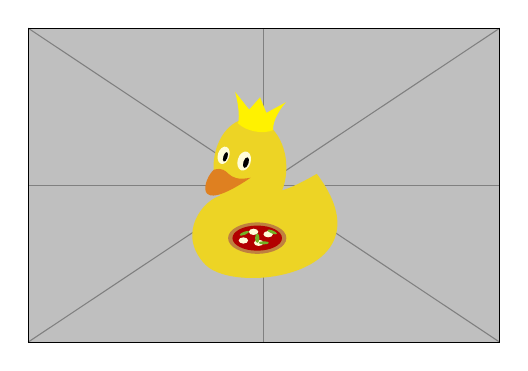
\begin{tikzpicture}
\clip (0,0) rectangle (6,4);
\node at (3,2) {%
\includegraphics[
width=6cm,height=4cm
]{example-image-duck}%
};
\jigsaw{6}{4}
\end{tikzpicture}}&
\scalebox{6}{🂨🂫}&
%\scalebox{3.3}{{\COE \Italy}}&
\scalebox{5}{\faChess}&
\scalebox{6}{\twemoji{tropical drink}}%
\\
(a)&(b)&(c)&(d)
\end{tabular}
\bigskip
\Huge

\onslide<2->{j}%
\onslide<3->{i}%
\onslide<4->{g}%
\onslide<5->{s}%
\onslide<6->{a}%
\onslide<7->{w}%


\large
\mbox{}\hfill{\tiny 0038}\,{\scriptsize \myaudio{./audio/quiz/answer_j.mp3}}
\end{frame}
%%%%%%%%%%%%%%%%%%%%%%%%%%%%%%%%%%%%%%%%%%%%%%%%%%
%% K
%%%%%%%%%%%%%%%%%%%%%%%%%%%%%%%%%%%%%%%%%%%%%%%%%%
\begin{frame}[plain]{Quiz}
\hypertarget{today_k}{}

 \large
{\small %
これからアルファベットを3つ順番に読みあげます。
聞こえたアルファベットを順番に小文字で書いてください。すると、ある単語になります。
その意味を表すものを選んでください
}\\
\mbox{}\hfill{\tiny 0043}\,{\scriptsize \myaudio{./audio/quiz/quiz_k.mp3}}

\bigskip

\centering
\newfontfamily{\COE}{CountriesOfEurope}
\begin{tabular}{c@{   }c@{   }c@{   }c}
\scalebox{5}{\twemoji{palm tree}}&
\scalebox{3}{\faCoffee}&
%\scalebox{3.3}{{\COE \Italy}}&
\fcKiteA{.1}{gray!80}{.2}&
\fcKey{.1}{gray!80}{.2}%
\\
(a)&(b)&(c)&(d)
\end{tabular}
\bigskip
\Huge

\onslide<2->{k}%
\onslide<3->{e}%
\onslide<4->{y}%
\hspace{10pt}%
\visible<5->{\textipa{/k\'\i:/}}

\large
\mbox{}\hfill{\tiny 0037}\,{\scriptsize \myaudio{./audio/quiz/answer_k.mp3}}
\end{frame}
%%%%%%%%%%%%%%%%%%%%%%%%%%%%%%%%%%%%%%%%%%%%%%%%%%
%% L
%%%%%%%%%%%%%%%%%%%%%%%%%%%%%%%%%%%%%%%%%%%%%%%%%%
\begin{frame}[plain]{Quiz}
\hypertarget{today_l}{}

 \large
{\small %
これからアルファベットを5つ順番に読みあげます。
聞こえたアルファベットを順番に小文字で書いてください。すると、ある単語になります。
その意味を表すものを選んでください
}\\
\mbox{}\hfill{\tiny 0054}\,{\scriptsize \myaudio{./audio/quiz/quiz_l.mp3}}

\bigskip

\centering
\newfontfamily{\COE}{CountriesOfEurope}
\begin{tabular}{c@{   }c@{   }c@{   }c}
\scalebox{5}{\twemoji{lemon}}&
\scalebox{5}{\twemoji{orange}}&
%\scalebox{3.3}{{\COE \Italy}}&
\scalebox{5}{\twemoji{lollipop}}&
\scalebox{5}{\twemoji{banana}}
\\
(a)&(b)&(c)&(d)
\end{tabular}
\bigskip
\Huge

\onslide<2->{l}%
\onslide<3->{e}%
\onslide<4->{m}%
\onslide<5->{o}%
\onslide<6->{n}%

\large
\mbox{}\hfill{\tiny 0037}\,{\scriptsize \myaudio{./audio/quiz/answer_l.mp3}}
\end{frame}
%%%%%%%%%%%%%%%%%%%%%%%%%%%%%%%%%%%%%%%%%%%%%%%%%%
\begin{frame}[plain]{檸檬}

\raggedleft

\includegraphics[height=.9\textheight]{./images/lemon.jpg}

\vspace*{-8pt}
\tiny
``Lemons and Limes, Fresh Fruit Color'' by moonjazz is licensed under CC BY 2.0.\\
To view a copy of this license, visit \url{https://creativecommons.org/licenses/by/2.0/?ref=openverse}.

\end{frame}
%%%%%%%%%%%%%%%%%%%%%%%%%%%%%%%%%%%%%%%%%%%%%%%%%%
%%%%%%%%%%%%%%%%%%%%%%%%%%%%%%%%%%%%%%%%%%%%%%%%%%
%% M
%%%%%%%%%%%%%%%%%%%%%%%%%%%%%%%%%%%%%%%%%%%%%%%%%%
\begin{frame}[plain]{Quiz}
\hypertarget{today_m}{}

 \large
{\small %
これからアルファベットを4つ順番に読みあげます。
聞こえたアルファベットを順番に小文字で書いてください。すると、ある単語になります。
その意味を表すものを選んでください
}\\
\mbox{}\hfill{\tiny 0048}\,{\scriptsize \myaudio{./audio/quiz/quiz_m.mp3}}

\bigskip

\centering
\newfontfamily{\COE}{CountriesOfEurope}
\begin{tabular}{c@{   }c@{   }c@{   }c}
\scalebox{5}{\twemoji{bubble tea}}&
\scalebox{5}{\twemoji{glass of milk}}&
%\scalebox{3.3}{{\COE \Italy}}&
\scalebox{5}{\twemoji{green apple}}&
\scalebox{5}{\twemoji{watermelon}}
\\
(a)&(b)&(c)&(d)
\end{tabular}
\bigskip
\Huge

\onslide<2->{m}%
\onslide<3->{i}%
\onslide<4->{l}%
\onslide<5->{k}%

\large
\mbox{}\hfill{\tiny 0037}\,{\scriptsize \myaudio{./audio/quiz/answer_m.mp3}}
\end{frame}
%%%%%%%%%%%%%%%%%%%%%%%%%%%%%%%%%%%%%%%%%%%%%%%%%%
%% N
%%%%%%%%%%%%%%%%%%%%%%%%%%%%%%%%%%%%%%%%%%%%%%%%%%
\begin{frame}[plain]{Quiz}
\hypertarget{today_n}{}

 \large
{\small %
これからアルファベットを8つ順番に読みあげます。
聞こえたアルファベットを順番に小文字で書いてください。すると、ある単語になります。
その意味を表すものを選んでください
}\\
\mbox{}\hfill{\tiny 0111}\,{\scriptsize \myaudio{./audio/quiz/quiz_n.mp3}}

\bigskip

\centering
\newfontfamily{\COE}{CountriesOfEurope}
\begin{tabular}{c@{   }c@{   }c@{   }c}
%\scalebox{5}{\twemoji{pencil}}&
\scalebox{3}{\ding{46}}&
\scalebox{5}{\twemoji{glass of milk}}&
%\scalebox{3.3}{{\COE \Italy}}&
\scalebox{5}{\twemoji{pen}}&
\scalebox{5}{\twemoji{notebook with decorative cover}}
\\
(a)&(b)&(c)&(d)
\end{tabular}

\bigskip

\Huge



\onslide<2->{n}%
\onslide<3->{o}%
\onslide<4->{t}%
\onslide<5->{e}%
\onslide<6->{b}%
\onslide<7->{o}%
\onslide<8->{o}%
\onslide<9->{k}%

\large
\mbox{}\hfill{\tiny 0039}\,{\scriptsize \myaudio{./audio/quiz/answer_n.mp3}}
\end{frame}
%%%%%%%%%%%%%%%%%%%%%%%%%%%%%%%%%%%%%%%%%%%%%%%%%%
%% O
%%%%%%%%%%%%%%%%%%%%%%%%%%%%%%%%%%%%%%%%%%%%%%%%%%
\begin{frame}[plain]{Quiz}
\hypertarget{today_o}{}

 \large
{\small %
これからアルファベットを5つ順番に読みあげます。
聞こえたアルファベットを順番に小文字で書いてください。すると、ある単語になります。
その意味を表すものを選んでください
}\\
\mbox{}\hfill{\tiny 0054}\,{\scriptsize \myaudio{./audio/quiz/quiz_o.mp3}}

\bigskip

\centering
\newfontfamily{\COE}{CountriesOfEurope}
\begin{tabular}{c@{   }c@{   }c@{   }c}
\scalebox{5}{\twemoji{tomato}}&
\scalebox{5}{\twemoji{broccoli}}&
%\scalebox{3.3}{{\COE \Italy}}&
\scalebox{5}{\twemoji{onion}}&
\scalebox{5}{\twemoji{eggplant}}
\\
(a)&(b)&(c)&(d)
\end{tabular}

\bigskip

\Huge

\onslide<2->{o}%
\onslide<3->{n}%
\onslide<4->{i}%
\onslide<5->{o}%
\onslide<6->{n}

\large
\mbox{}\hfill{\tiny 0037}\,{\scriptsize \myaudio{./audio/quiz/answer_o.mp3}}
\end{frame}
%%%%%%%%%%%%%%%%%%%%%%%%%%%%%%%%%%%%%%%%%%%%%%%%%%
%% P
%%%%%%%%%%%%%%%%%%%%%%%%%%%%%%%%%%%%%%%%%%%%%%%%%%
\begin{frame}[plain]{Quiz}
\hypertarget{today_p}{}

 \large
{\small %
これからアルファベットを5つ順番に読みあげます。
聞こえたアルファベットを順番に小文字で書いてください。すると、ある単語になります。
その意味を表すものを選んでください
}\\
\mbox{}\hfill{\tiny 0054}\,{\scriptsize \myaudio{./audio/quiz/quiz_p.mp3}}

\bigskip

\centering
\newfontfamily{\COE}{CountriesOfEurope}
\begin{tabular}{c@{   }c@{   }c@{   }c}
\scalebox{5}{\twemoji{strawberry}}&
\scalebox{5}{\twemoji{orange}}&
%\scalebox{3.3}{{\COE \Italy}}&
\scalebox{5}{\twemoji{banana}}&
\scalebox{5}{\twemoji{peach}}
\\
(a)&(b)&(c)&(d)
\end{tabular}

\bigskip

\Huge



\onslide<2->{p}%
\onslide<3->{e}%
\onslide<4->{a}%
\onslide<5->{c}%
\onslide<6->{h}

\large
\mbox{}\hfill{\tiny 0038}\,{\scriptsize \myaudio{./audio/quiz/answer_p.mp3}}
\end{frame}
%%%%%%%%%%%%%%%%%%%%%%%%%%%%%%%%%%%%%%%%%%%%%%%%%%
%% Q
%%%%%%%%%%%%%%%%%%%%%%%%%%%%%%%%%%%%%%%%%%%%%%%%%%
\begin{frame}[plain]{Quiz}
\hypertarget{today_q}{}

 \large
{\small %
これからアルファベットを5つ順番に読みあげます。
聞こえたアルファベットを順番に小文字で書いてください。すると、ある単語になります。
その意味を表すものを選んでください
}\\
\mbox{}\hfill{\tiny 0055}\,{\scriptsize \myaudio{./audio/quiz/quiz_q.mp3}}

\bigskip

\centering
\newfontfamily{\COE}{CountriesOfEurope}
\begin{tabular}{c@{   }c@{   }c@{   }c}
\scalebox{6}{🃋}&
\scalebox{6}{🂭}&
\scalebox{6}{🂾}&
%\scalebox{3.3}{{\COE \Italy}}&
\scalebox{6}{🃏}
\\
(a)&(b)&(c)&(d)
\end{tabular}

\bigskip

\Huge

\onslide<2->{q}%
\onslide<3->{u}%
\onslide<4->{e}%
\onslide<5->{e}%
\onslide<6->{n}

\large
\mbox{}\hfill{\tiny 0037}\,{\scriptsize \myaudio{./audio/quiz/answer_q.mp3}}
\end{frame}
%%%%%%%%%%%%%%%%%%%%%%%%%%%%%%%%%%%%%%%%%%%%%%%%%%
%% R
%%%%%%%%%%%%%%%%%%%%%%%%%%%%%%%%%%%%%%%%%%%%%%%%%%
\begin{frame}[plain]{Quiz}
\hypertarget{today_r}{}

 \large
{\small %
これからアルファベットを7つ順番に読みあげます。
聞こえたアルファベットを順番に小文字で書いてください。すると、ある単語になります。
その意味を表すものを選んでください
}\\
\mbox{}\hfill{\tiny 0106}\,{\scriptsize \myaudio{./audio/quiz/quiz_r.mp3}}

\bigskip

\centering

\begin{tabular}{c@{   }c@{   }c@{   }c}
\scalebox{6}{\twemoji{rainbow}}&
\scalebox{6}{\twemoji{cloud with snow}}&
\scalebox{6}{\twemoji{sun behind small cloud}}&
\scalebox{6}{\twemoji{cloud with lightning and rain}}
\\
(a)&(b)&(c)&(d)
\end{tabular}


\bigskip

\Huge

\onslide<2->{r}%
\onslide<3->{a}%
\onslide<4->{i}%
\onslide<5->{n}%
\onslide<6->{b}%
\onslide<7->{o}%
\onslide<8->{w}

\large
\mbox{}\hfill{\tiny 0038}\,{\scriptsize \myaudio{./audio/quiz/answer_r.mp3}}
\end{frame}

%%%%%%%%%%%%%%%%%%%%%%%%%%%%%%%%%%%%%%%%%%
%{
%  \usebackgroundtemplate{\includegraphics[width=\paperwidth]{./images/rainbow.jpg}}
%  \begin{frame}[t]
%    \frametitle{}
%\tiny
%
%\raggedleft
%  \textcolor{white}{``Brilliant double rainbow after a sudden rainstorm (explore)'' by Peggy2012CREATIVELENZ is licensed under CC BY 2.0.}\\
%   \textcolor{white}{To view a copy of this license, visit \url{https://creativecommons.org/licenses/by/2.0/?ref=openverse}.}
%  \end{frame}
%}
%%%%%%%%%%%%%%%%%%%%%%%%%%%%%%%%%%%%%%%%%%%%%%%%%%
%% S
%%%%%%%%%%%%%%%%%%%%%%%%%%%%%%%%%%%%%%%%%%%%%%%%%%
\begin{frame}[plain]{Quiz}
\hypertarget{today_s}{}

 \large
{\small %
これからアルファベットを10個、順番に読みあげます。
聞こえたアルファベットを順番に小文字で書いてください。すると、ある単語になります。
その意味を表すものを選んでください
}
\mbox{}\hfill{\tiny 0123}\,{\scriptsize \myaudio{./audio/quiz/quiz_s.mp3}}

\bigskip

\centering

\begin{tabular}{c@{   }c@{   }c@{   }c}
\scalebox{6}{\twemoji{shaved ice}}&
\scalebox{6}{\twemoji{tangerine}}&
\scalebox{6}{\twemoji{cup with straw}}&
\scalebox{6}{\twemoji{strawberry}}
\\
(a)&(b)&(c)&(d)
\end{tabular}


\bigskip

\Huge

\onslide<2->{s}%
\onslide<3->{t}%
\onslide<4->{r}%
\onslide<5->{a}%
\onslide<6->{w}%
\onslide<7->{b}%
\onslide<8->{e}%
\onslide<9->{r}%
\onslide<10->{r}%
\onslide<11->{y}

\large
\mbox{}\hfill{\tiny 0040}\,{\scriptsize \myaudio{./audio/quiz/answer_s.mp3}}
\end{frame}
%%%%%%%%%%%%%%%%%%%%%%%%%%%%%%%%%%%%%%%%%
{
  \usebackgroundtemplate{\includegraphics[width=\paperwidth]{./images/berry.jpg}}
  \begin{frame}[b]
    \frametitle{}
\tiny

\raggedleft
  \textcolor{white}{``Strawberries''by Hades2k is licensed under CC BY-SA 2.0.}\\
   \textcolor{white}{To view a copy of this license, visit \url{https://creativecommons.org/licenses/by-sa/2.0/?ref=openverse}.}
  \end{frame}
}
%%%%%%%%%%%%%%%%%%%%%%%%%%%%%%%%%%%%%%%%%%%%%%%%%%
%% T
%%%%%%%%%%%%%%%%%%%%%%%%%%%%%%%%%%%%%%%%%%%%%%%%%%
\begin{frame}[plain]{Quiz}
\hypertarget{today_t}{}

 \large
{\small %
これからアルファベットを5つ順番に読みあげます。
聞こえたアルファベットを順番に小文字で書いてください。すると、ある単語になります。
その意味を表すものを選んでください
}\\
\mbox{}\hfill{\tiny 0054}\,{\scriptsize \myaudio{./audio/quiz/quiz_t.mp3}}

\bigskip

\centering

\begin{tabular}{c@{   }c@{   }c@{   }c}
\scalebox{6}{\twemoji{zebra}}&
\scalebox{6}{\twemoji{tiger face}}&
\scalebox{6}{\twemoji{lion}}&
\scalebox{6}{\twemoji{T-Rex}}
\\
(a)&(b)&(c)&(d)
\end{tabular}


\bigskip

\Huge

\onslide<2->{t}%
\onslide<3->{i}%
\onslide<4->{g}%
\onslide<5->{e}%
\onslide<6->{r}%

\large
\mbox{}\hfill{\tiny 0038}\,{\scriptsize \myaudio{./audio/quiz/answer_t.mp3}}
\end{frame}
%%%%%%%%%%%%%%%%%%%%%%%%%%%%%%%%%%%%%%%%%%%%%%%%%%
%% U
%%%%%%%%%%%%%%%%%%%%%%%%%%%%%%%%%%%%%%%%%%%%%%%%%%
\begin{frame}[plain]{Quiz}
\hypertarget{today_u}{}

 \large
{\small %
これからアルファベットを8つ順番に読みあげます。
聞こえたアルファベットを順番に小文字で書いてください。すると、ある単語になります。
その意味を表すものを選んでください
}
\mbox{}\hfill{\tiny 0112}\,{\scriptsize \myaudio{./audio/quiz/quiz_u.mp3}}

\bigskip

\centering

\begin{tabular}{c@{   }c@{   }c@{   }c}
\scalebox{6}{\twemoji{umbrella}}&
\scalebox{6}{\twemoji{toothbrush}}&
\scalebox{6}{\twemoji{envelope}}&
\scalebox{6}{\twemoji{eyeglasses}}
\\
(a)&(b)&(c)&(d)
\end{tabular}


\bigskip

\Huge

\onslide<2->{u}%
\onslide<3->{m}%
\onslide<4->{b}%
\onslide<5->{r}%
\onslide<6->{e}%
\onslide<7->{l}%
\onslide<8->{l}%
\onslide<9->{a}%

\large
\mbox{}\hfill{\tiny 0039}\,{\scriptsize \myaudio{./audio/quiz/answer_u.mp3}}
\end{frame}
%%%%%%%%%%%%%%%%%%%%%%%%%%%%%%%%%%%%%%%%%%%%%%%%%%
%% V
%%%%%%%%%%%%%%%%%%%%%%%%%%%%%%%%%%%%%%%%%%%%%%%%%%
\begin{frame}[plain]{Quiz}
\hypertarget{today_v}{}

 \large
{\small %
これからアルファベットを9つ順番に読みあげます。
聞こえたアルファベットを順番に小文字で書いてください。すると、ある単語になります。
その意味を表すものを選んでください
}
\mbox{}\hfill{\tiny 0117}\,{\scriptsize \myaudio{./audio/quiz/quiz_v.mp3}}

\bigskip

\centering

\begin{tabular}{c@{   }c@{   }c@{   }c}
\scalebox{6}{\twemoji{sandwich}}&
\scalebox{3.5}{\twemoji{tomato}\twemoji{cucumber}}&
\scalebox{6}{\twemoji{rice ball}}&
\scalebox{6}{\twemoji{curry rice}}
\\
(a)&(b)&(c)&(d)
\end{tabular}


\bigskip

\Huge

\onslide<2->{v}%
\onslide<3->{e}%
\onslide<4->{g}%
\onslide<5->{e}%
\onslide<6->{t}%
\onslide<7->{a}%
\onslide<8->{b}%
\onslide<9->{l}%
\onslide<10->{e}

\large
\mbox{}\hfill{\tiny 0039}\,{\scriptsize \myaudio{./audio/quiz/answer_v.mp3}}
\end{frame}
%%%%%%%%%%%%%%%%%%%%%%%%%%%%%%%%%%%%%%%%%%%%%%%%%%
%% W
%%%%%%%%%%%%%%%%%%%%%%%%%%%%%%%%%%%%%%%%%%%%%%%%%%
\begin{frame}[plain]{Quiz}
\hypertarget{today_w}{}

 \large
{\small %
これからアルファベットを5つ順番に読みあげます。
聞こえたアルファベットを順番に小文字で書いてください。すると、ある単語になります。
その意味を表すものを選んでください
}\\
\mbox{}\hfill{\tiny 0055}\,{\scriptsize \myaudio{./audio/quiz/quiz_w.mp3}}

\bigskip

\centering

\begin{tabular}{c@{   }c@{   }c@{   }c}
\scalebox{6}{\twemoji{spouting whale}}&
\rotatebox{90}{\scalebox{6}{\twemoji{spoon}}}&
\scalebox{6}{\twemoji{watch}}&
\scalebox{6}{\twemoji{volleyball}}
\\
(a)&(b)&(c)&(d)
\end{tabular}


\bigskip

\Huge

\onslide<2->{w}%
\onslide<3->{a}%
\onslide<4->{t}%
\onslide<5->{c}%
\onslide<6->{h}%

\large
\mbox{}\hfill{\tiny 0038}\,{\scriptsize \myaudio{./audio/quiz/answer_w.mp3}}
\end{frame}
%%%%%%%%%%%%%%%%%%%%%%%%%%%
%%%%%%%%%%%%%%%%%%%%%%%%%%%%%%%%%%%%%%%%%%%%%%%%%%
%% X
%%%%%%%%%%%%%%%%%%%%%%%%%%%%%%%%%%%%%%%%%%%%%%%%%%
\begin{frame}[plain]{Quiz}
\hypertarget{today_x}{}

 \large
{\small %
これからアルファベットを4つ順番に読みあげます。
聞こえたアルファベットを順番に書いてください。ただし最初の1文字だけは大文字で書いてください。ある単語になります。
その意味を表すものを選んでください
}\\
\mbox{}\hfill{\tiny 0048}\,{\scriptsize \myaudio{./audio/quiz/quiz_x.mp3}}

\bigskip

\centering

\begin{tabular}{c@{   }c@{   }c@{   }c}
\scalebox{6}{\twemoji{Japanese dolls}}&
\scalebox{6}{\twemoji{pine decoration}}&
\scalebox{6}{\twemoji{jack-o-lantern}}&
\scalebox{6}{\twemoji{Christmas tree}}
\\
(a)&(b)&(c)&(d)
\end{tabular}


\bigskip

\Huge

\onslide<2->{X}%
\onslide<3->{m}%
\onslide<4->{a}%
\onslide<5->{s}
\onslide<6->{{\small ($=\text{Christmas}$)}}

\hfill\onslide<7->{{\small X'masはまちがい}}

\large
\mbox{}\hfill{\tiny 0039}\,{\scriptsize \myaudio{./audio/quiz/answer_x.mp3}}
\end{frame}
%%%%%%%%%%%%%%%%%%%%%%%%%%%%%
\begin{frame}[plain]{どう発音していますか}
\LARGE
\begin{enumerate}
 \item \kenten{く}りごはん(栗ごはん)\\
\mbox{}
 \item しゃっ\kenten{く}り
\end{enumerate}
 
\end{frame}

%%%%%%%%%%%%%%%%%%%%%%%%%%%%%%%%%%%%%%%%%%%%%%%%%%
%% Y
%%%%%%%%%%%%%%%%%%%%%%%%%%%%%%%%%%%%%%%%%%%%%%%%%%
\begin{frame}[plain]{Quiz}
\hypertarget{today_y}{}

 \large
{\small %
これからアルファベットを6つ順番に読みあげます。
聞こえたアルファベットを順番に小文字で書いてください。すると、ある単語になります。
その意味を表すものを選んでください
}\\
\mbox{}\hfill{\tiny 0101}\,{\scriptsize \myaudio{./audio/quiz/quiz_y.mp3}}

\bigskip

\centering

\begin{tabular}{c@{   }c@{   }c@{   }c}

\begin{tikzpicture}
    \filldraw[fill=NavyBlue] (1.5,0) rectangle (2.5,1); % 青塗りの正方形
\end{tikzpicture}&

\begin{tikzpicture}
    \filldraw[fill=Maroon] (1.5,0) rectangle (2.5,1); % 青塗りの正方形
\end{tikzpicture}&
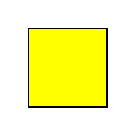
\begin{tikzpicture}
    \filldraw[fill=Yellow] (1.5,0) rectangle (2.5,1); % 青塗りの正方形
\end{tikzpicture}&

\begin{tikzpicture}
    \filldraw[fill=OliveGreen] (1.5,0) rectangle (2.5,1); % 青塗りの正方形
\end{tikzpicture}
\\
(a)&(b)&(c)&(d)
\end{tabular}


\bigskip

\Huge

\onslide<2->{y}%
\onslide<3->{e}%
\onslide<4->{l}%
\onslide<5->{l}%
\onslide<6->{o}%
\onslide<7->{w}

\large
\mbox{}\hfill{\tiny 0038}\,{\scriptsize \myaudio{./audio/quiz/answer_y.mp3}}
\end{frame}
%%%%%%%%%%%%%%%%%%%%%%
% 背景色を黒に変更
\setbeamercolor{background canvas}{bg=black}
\begin{frame}
\centering
  \textcolor{white}{\Huge\bfseries Today's Quiz}

\vfill

 \textcolor{white}{\Huge\bfseries 2024-09-13}

\end{frame}
\setbeamercolor{background canvas}{bg=}
%%%%%%%%%%%%%%%%%%%%%%%%%%
%%%%%%%%%%%%%%%%%%%%%%%%%%%%%%%%%%%%%%%%%%%%%%%%%%
%% Z
%%%%%%%%%%%%%%%%%%%%%%%%%%%%%%%%%%%%%%%%%%%%%%%%%%
\begin{frame}[plain]{Quiz}
\hypertarget{today_z}{}

 \large
{\small %
これからアルファベットを4つ順番に読みあげます。
聞こえたアルファベットを順番に小文字で書いてください。すると、ある単語になります。
その意味を表すものを選んでください
}
\mbox{}\hfill{\tiny 0048}\,{\scriptsize \myaudio{./audio/quiz/quiz_z.mp3}}

\bigskip

\centering

\begin{tabular}{c@{   }c@{   }c@{   }c}
\scalebox{2}{$1+2$}&
\scalebox{2}{$3-2$}&
\scalebox{2}{$\frac{1}{2}-0.5$}&
\scalebox{2}{$1-0$}
\\[15pt]
(a)&(b)&(c)&(d)
\end{tabular}

\bigskip

\Huge

\onslide<2->{z}%
\onslide<3->{e}%
\onslide<4->{r}%
\onslide<5->{o}

\large
\mbox{}\hfill{\tiny 0038}\,{\scriptsize \myaudio{./audio/quiz/answer_z.mp3}}
\end{frame}
%%%%%%%%%%%%%%%%%%%%%%%%%%%%%%%%%%%%%%%%%%%%%%%%%%%%%%%%%%%%%%%%%%
\end{document}
